\allowdisplaybreaks

\begin{document}
    \title{Physik IV Übungsblatt 8}
    \author{  
    Tobias Rücker\\
    \texorpdfstring{\href{mailto:tobias.ruecker@tu-dortmund.de}{tobias.ruecker@tu-dortmund.de}
    \and}{,} 
    Paul Störbrock\\
    \texorpdfstring{\href{mailto:paul.stoerbrock@tu-dortmund.de}{paul.stoerbrock@tu-dortmund.de}}{}
    }
\maketitle
\center{\Large Abgabegruppe: \textbf{4H}}
\thispagestyle{empty}

\newpage
\tableofcontents
\thispagestyle{empty}
\newpage

\setcounter{page}{1}

\section{Aufgabe 1}

    \begin{figure}[H]
        \centering
        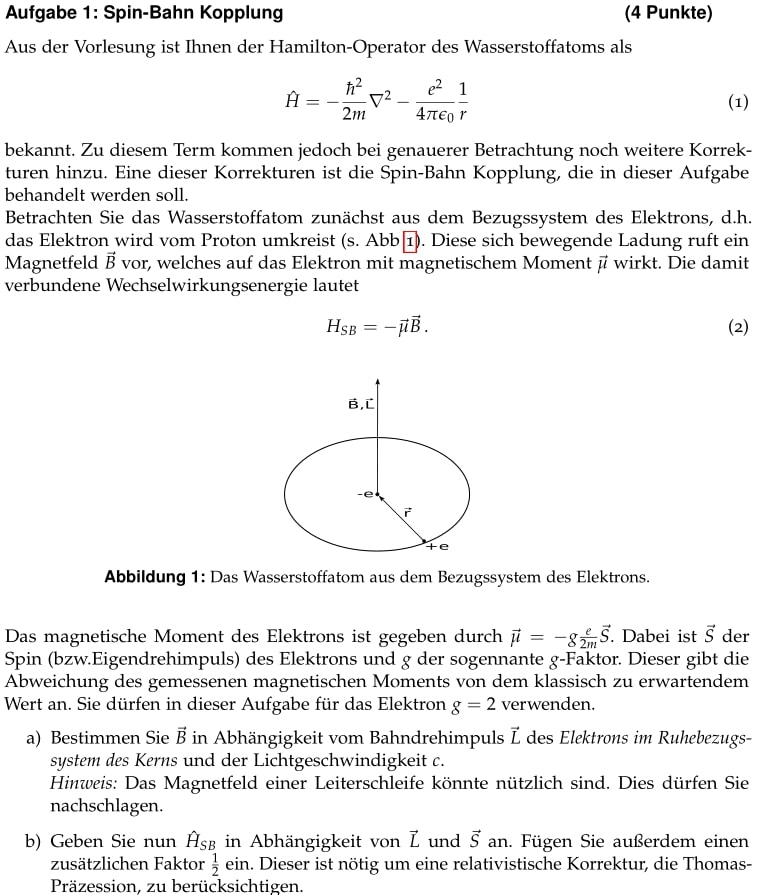
\includegraphics[width=\textwidth]{images/Aufgabe1a.jpg}
        \label{fig:1}
    \end{figure}

    \begin{figure}[H]
        \centering
        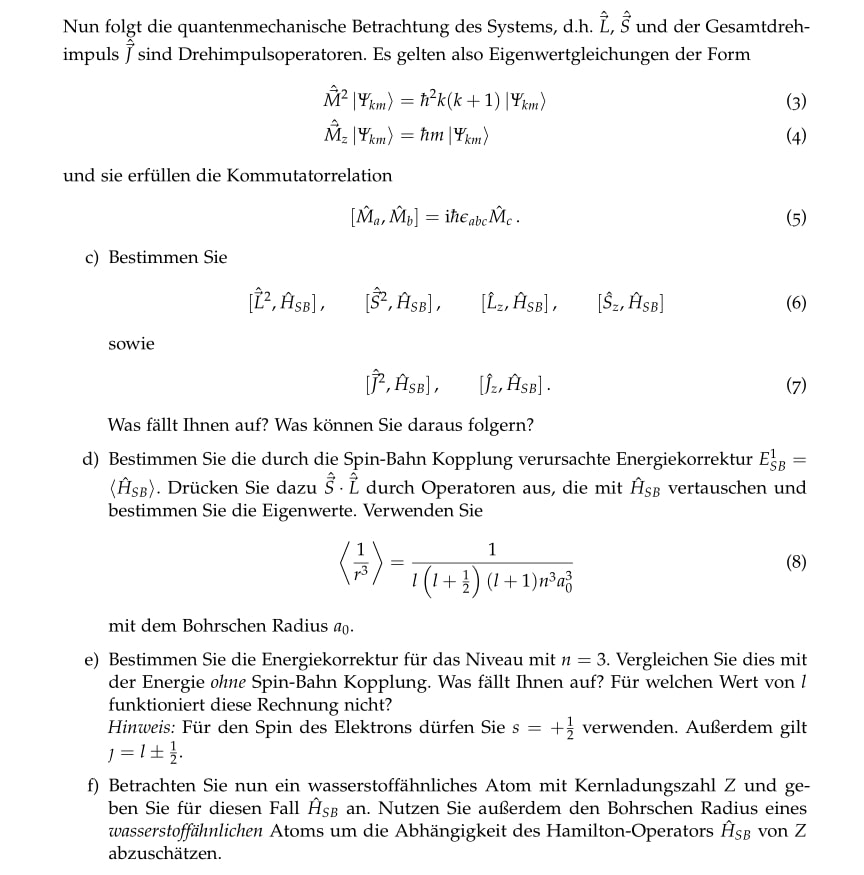
\includegraphics[width=\textwidth]{images/Aufgabe1b.jpg}
        \label{fig:2}
    \end{figure}

    \subsection{a)}

    \subsection{b)}

    \subsection{c)}

    \subsection{d)}

    \subsection{e)}

    \subsection{f)}

\section{Aufgabe 2}

    \begin{figure}[H]
        \centering
        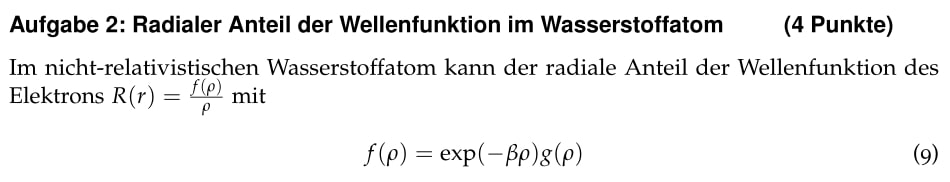
\includegraphics[width=\textwidth]{images/Aufgabe2a.jpg}
        \label{fig:3}
    \end{figure}

    \begin{figure}[H]
        \centering
        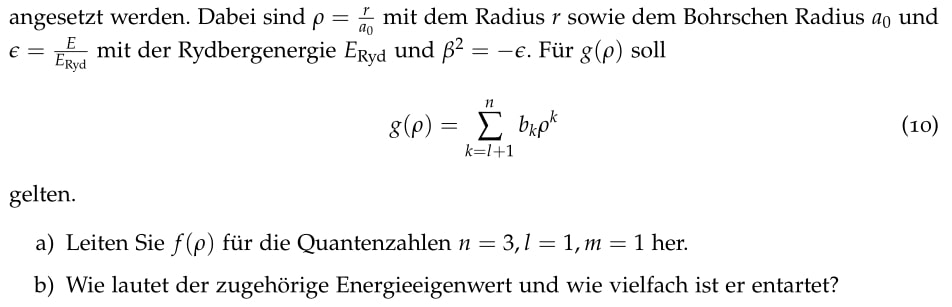
\includegraphics[width=\textwidth]{images/Aufgabe2b.jpg}
        \label{fig:4}
    \end{figure}

    \subsection{a)}

    \subsection{b)}

\section{Aufgabe 3}

    \begin{figure}[H]
        \centering
        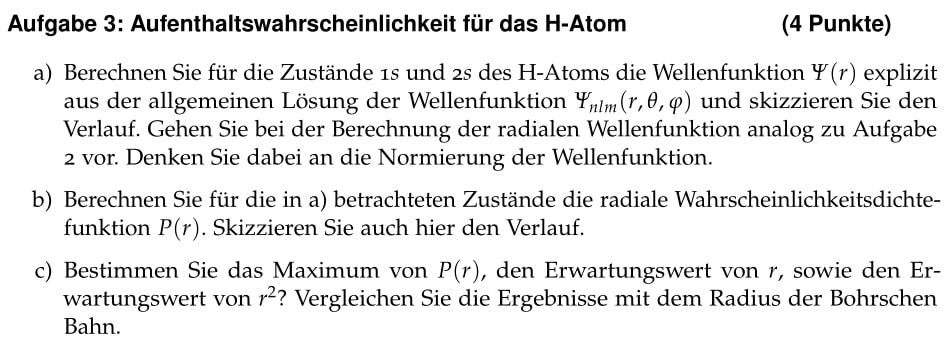
\includegraphics[width=\textwidth]{images/Aufgabe3.jpg}
        \label{fig:5}
    \end{figure}

    \subsection{a)}

    \subsection{b)}

    \subsection{c)}

\section{Aufgabe 4}

    \begin{figure}[H]
        \centering
        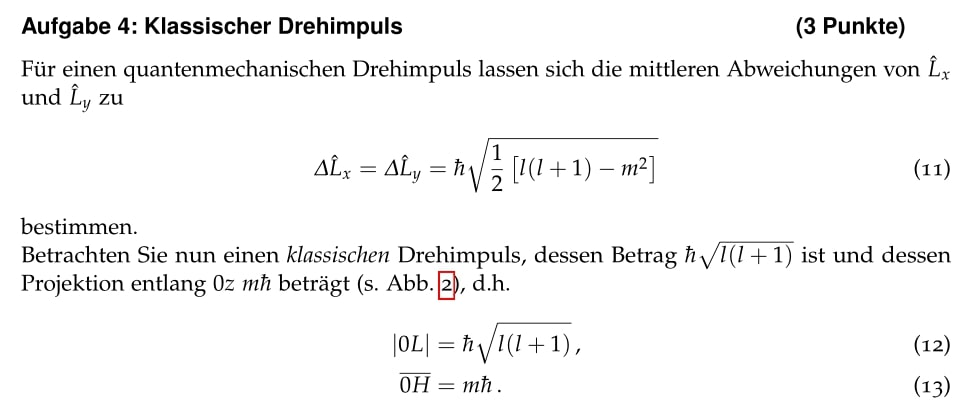
\includegraphics[width=\textwidth]{images/Aufgabe4a.jpg}
        \label{fig:6}
    \end{figure}

    \begin{figure}[H]
        \centering
        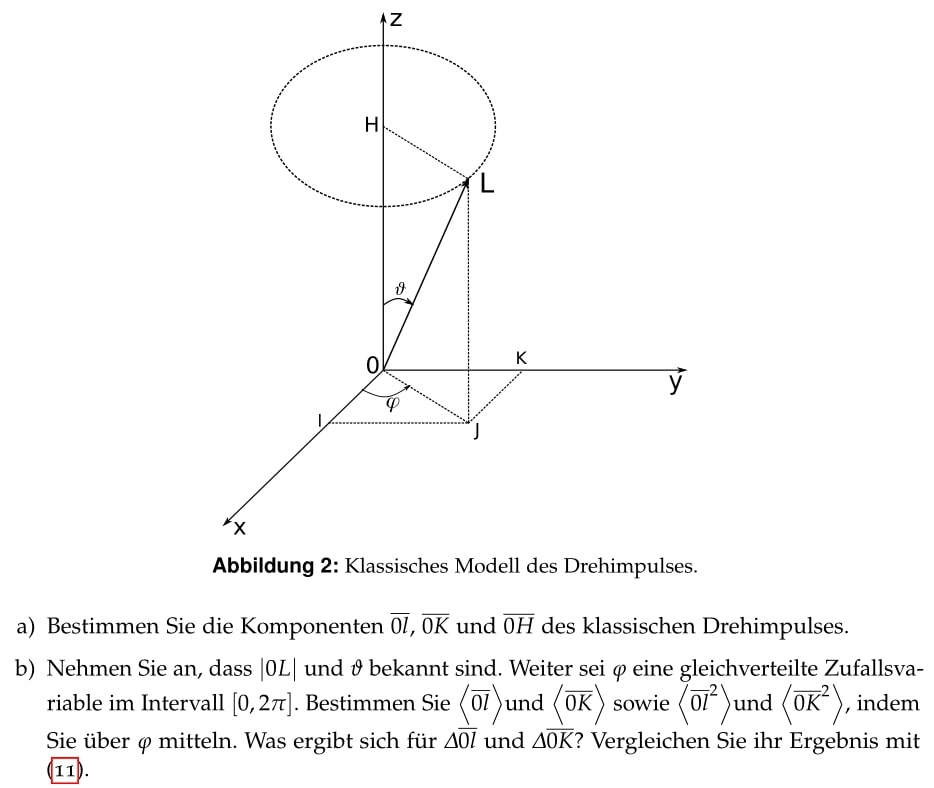
\includegraphics[width=\textwidth]{images/Aufgabe4b.jpg}
        \label{fig:7}
    \end{figure}

    \subsection{a)}

    \subsection{b)}









\end{document}